% begin module volumes-ex2
\begin{frame}
\begin{example}
Find the volume of the solid obtained by rotating about the $x$-axis the region under the curve $y = \sqrt{x}$ from $0$ to $1$.
\begin{itemize}
\item<13->  The cross-sections of this solid are all circles.
\item<15->  The circular cross-section through the point $(x, 0)$ has radius $\sqrt{x}$.
\item<10->  The area of the cross-section is \alertNoH{10,11}{$A(x) =  \fcAnswerNoH{11}{\pi (\sqrt{x})^2  = \pi x.}$}
\item<13->  The volume of a single approximating section is $A(x) \Delta x = \pi x \ \Delta x$.
\item<14->  The solid lies between $0$ and $1$, so its volume is
\end{itemize}
\begin{columns}[c]
\column{.4\textwidth}
\begin{center}
\psset{xunit=1cm, yunit=1cm}
\begin{pspicture}(-1,-1)(1,1)
\tiny%
\renewcommand{\fcScreenStyle}{x}%
\renewcommand{\fcScreen}{[0 0 -1] 0}%
\renewcommand{\fcIterationsU}{4}%
\fcBoundingBox{-2}{-2}{2}{2}
\only<3->{\renewcommand{\fcScreen}{[-0.05 -0.05 -1] 0}}%
\only<4->{\renewcommand{\fcScreen}{[-0.1 -0.1 -1] 0}}%
\only<5->{\renewcommand{\fcScreen}{[-0.15 -0.15 -1] 0}}%
\only<6->{\renewcommand{\fcScreen}{[-0.2 -0.2 -1] 0}}%
\only<7->{\renewcommand{\fcScreen}{[-0.25 -0.25 -1] 0}}%
\fcStartIIIdScene%
\only<3->{\fcPutIIId{[-0.1 -0.1 1.6]}{$z$}}%
\fcPutIIId{[0 1.6 ]}{$y$}%
\fcPutIIId{[1.6 0 0]}{$x$}%
\fcAxesIIIdFullInScene{1.5}{1.5}{1.5}%
\only<handout:0|9>{\fcSurfaceInScene[iterationsV=3, iterationsU=3, arrows=(none), linecolor=black, linewidth=0.3]{0.01 }{0}{1}{40 3 mul}{[u u sqrt v cos mul u sqrt v sin mul]}{}%
\fcSurfaceInScene[iterationsV=3, iterationsU=1]{0.04}{ 0}{ 1}{ 40 3 mul}{[1 v cos u mul v sin u mul]}{}%
}%
\only<handout:0|10>{\fcSurfaceInScene[iterationsV=5, iterationsU=3, arrows=(none), linecolor=black, linewidth=0.3]{0.01 }{0}{1}{40 5 mul}{[u u sqrt v cos mul u sqrt v sin mul]}{}%
\fcSurfaceInScene[iterationsV=5, iterationsU=1]{0.04}{0}{1}{40 5 mul}{[1 v cos u mul v sin u mul]}{}%
}%
\only<handout:0|11>{\fcSurfaceInScene[iterationsV=7, iterationsU=3, arrows=(none), linecolor=black, linewidth=0.3]{0.04 }{0}{1}{40 7 mul}{[u u sqrt v cos mul u sqrt v sin mul]}{}%
\fcSurfaceInScene[iterationsV=7, iterationsU=1]{0.04}{0}{1}{40 7 mul}{[1 v cos u mul v sin u mul]}{}%
}%
\only<handout:1|12,13>{\fcSurfaceInScene[iterationsV=9, iterationsU=3, arrows=(none), linecolor=black, linewidth=0.3]{0.01 }{0}{1}{40 9 mul}{[u u sqrt v cos mul u sqrt v sin mul]}{}%
\fcSurfaceInScene[iterationsV=9, iterationsU=1]{0.04}{0}{1}{40 9 mul}{[1 v cos u mul v sin u mul]}{}%
}%
\only<handout:0|13>{\fcCurveIIIdInScene[arrows=(none), linewidth=2, linecolor=blue]{0 }{360 }{[2 3 div t cos 2 3 div sqrt mul t sin 0.6 sqrt mul]}}
\only<handout:1|14->{\fcSurfaceInScene[arrows=(none), linecolor=blue, colorUV=cyan, iterationsV=3, iterationsU=1]{0.04}{0}{2 3 div sqrt}{40 9 mul}{[2 3 div v cos u mul v sin u mul]}{}}%
\only<2->{\fcCurveIIIdInScene[arrows=(none),linecolor=\fcColorGraph]{0}{1}{[t t sqrt 0]}}%
\only<8->{\fcCurveIIIdInScene[arrows=->, linewidth=2, linecolor=cyan]{-90 }{120 }{[-1.3 t cos 0.4 mul t sin 0.4 mul]}%
\fcCurveIIIdInScene[arrows=(none), linewidth=2, linecolor=cyan]{120 }{245 }{[-1.3 t cos 0.4 mul t sin 0.4 mul]}%
}%
\fcFinishIIIdScene[true]%
\end{pspicture}
%\only<handout:0| 1>{%
%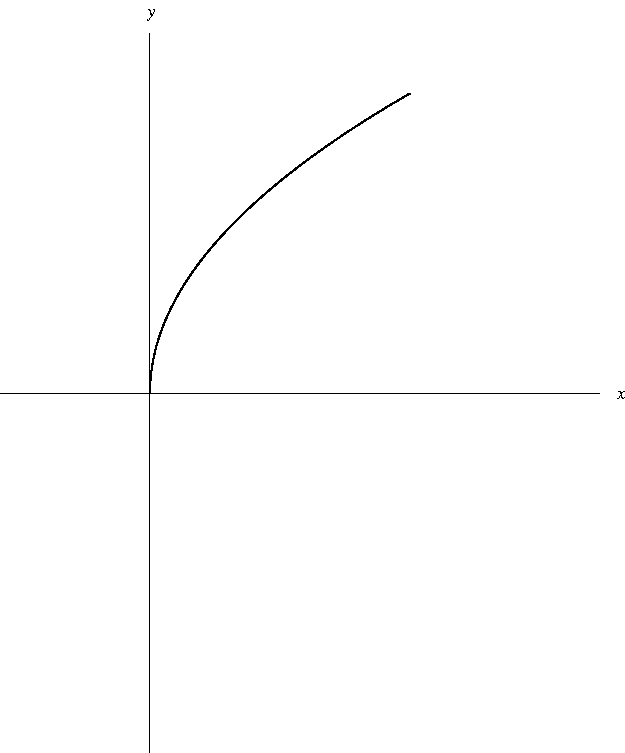
\includegraphics[height=3.5cm]{volumes/pictures/06-02-ex2a.pdf} %
%}%
%\only<handout:0| 2>{%
%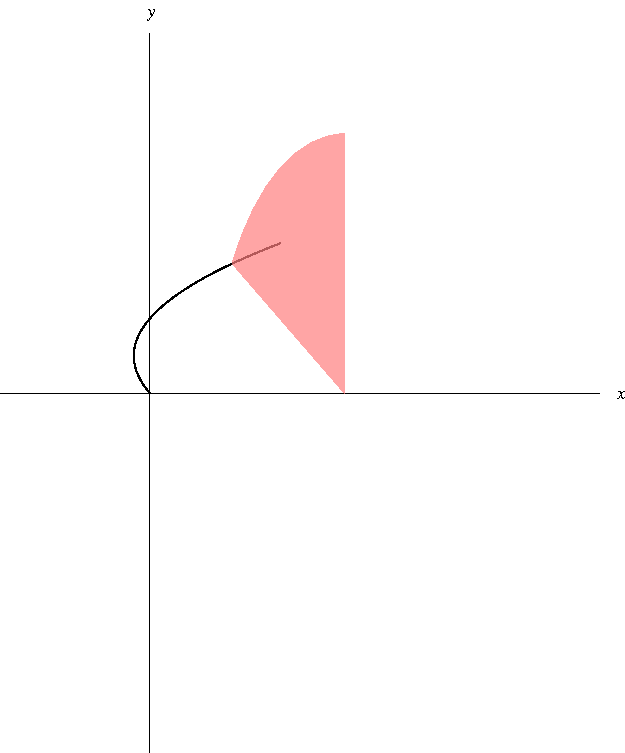
\includegraphics[height=3.5cm]{volumes/pictures/06-02-ex2b.pdf} %
%}%
%\only<handout:0| 3>{%
%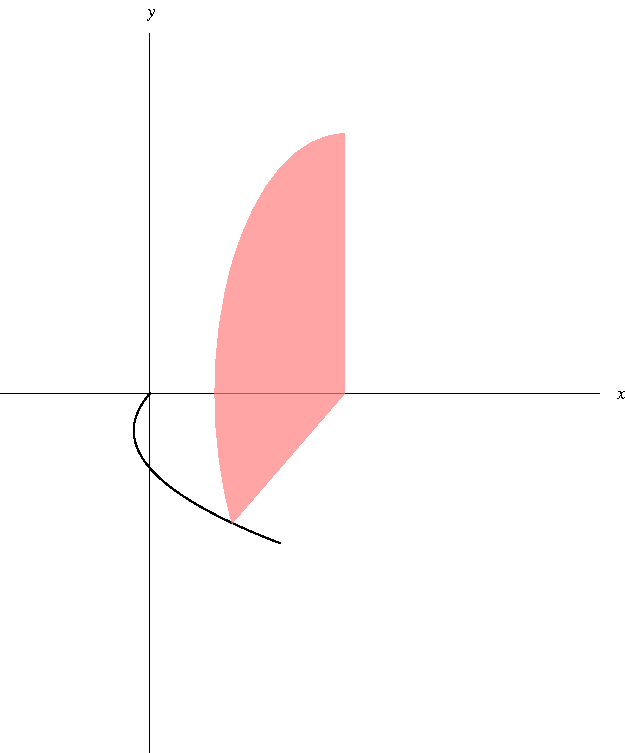
\includegraphics[height=3.5cm]{volumes/pictures/06-02-ex2c.pdf} %
%}%
%\only<handout:0| 4>{%
%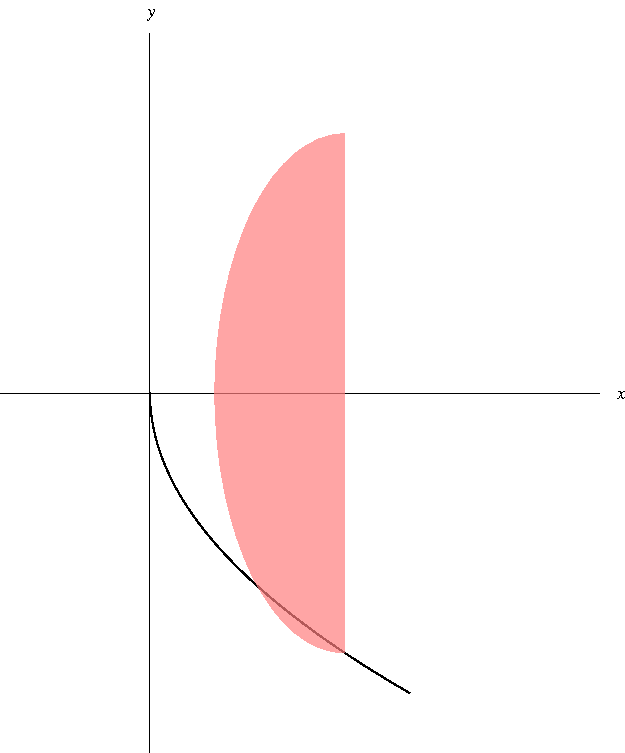
\includegraphics[height=3.5cm]{volumes/pictures/06-02-ex2d.pdf} %
%}%
%\only<handout:0| 5>{%
%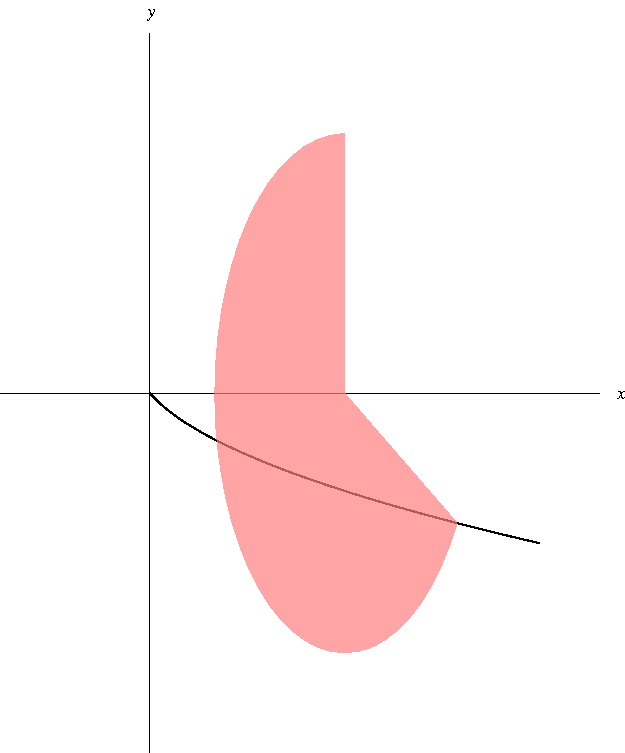
\includegraphics[height=3.5cm]{volumes/pictures/06-02-ex2e.pdf} %
%}%
%\only<handout:0| 6>{%
%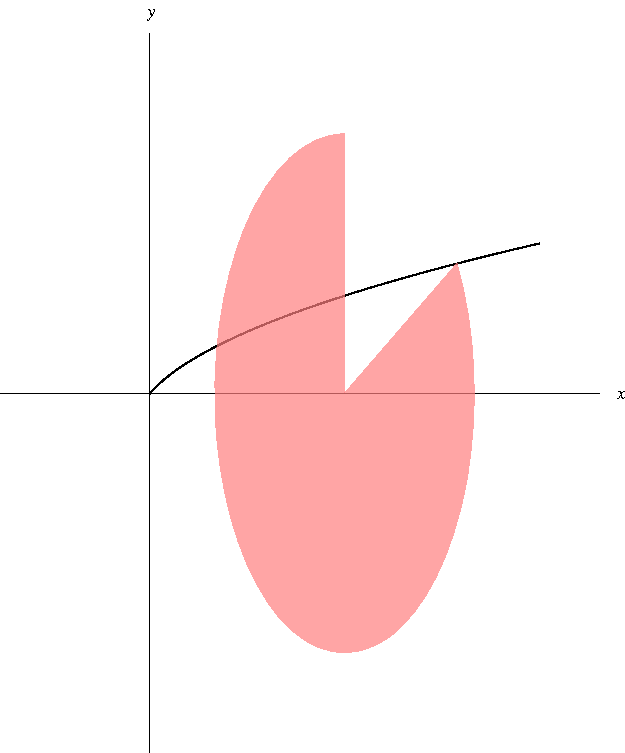
\includegraphics[height=3.5cm]{volumes/pictures/06-02-ex2f.pdf} %
%}%
%\only<7->{%
%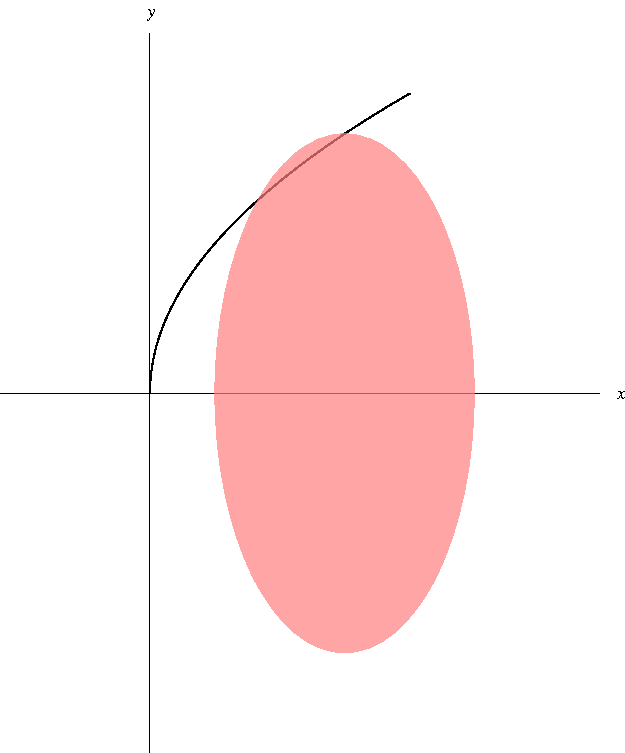
\includegraphics[height=3.5cm]{volumes/pictures/06-02-ex2g.pdf} %
%}%
\end{center}
\column{.6\textwidth}
\abovedisplayskip=0pt
\belowdisplayskip=0pt
\abovedisplayshortskip=0pt
\belowdisplayshortskip=0pt
\begin{align*}
\uncover<14->{%
V%
}%
& \uncover<14->{ = } %
\uncover<14->{%
\int_0^1 A(x) \ \diff x%
}%
 \uncover<15->{ = } %
\uncover<15->{%
\int_0^1 \pi x \ \diff x%
}\\%
& \uncover<16->{ = } %
\uncover<16->{%
\left[ \pi \frac{x^2}{2}\right]_0^1%
}%
 \uncover<17->{ = } %
\uncover<17->{%
\frac{\pi}{2}%
}%
\end{align*}
\end{columns}
\end{example}
\end{frame}
% end module volumes-ex2
